\section{How to control a detector?}

Data acquisition, parameter monitoring, control, logging, and storage are mandatory tasks for every experimental setup. The previously mentioned tasks become even more important and challenging in an environment of heavy ionizing radiation. Moreover, automation of different processes in form of e.g. finite state machines ensures that the transition between states of the detector is performed in a controlled and safe fashion. Ambient conditions and other process variables monitoring provide also important insights into the detector's performance.  To ease the use and implementation of a control system, a fairly novel approach was used. It is primarily based on the \footnote{Containerization is the packaging of software code with just the operating system libraries and dependencies required to run the code.}{containerization} of different applications used to monitor and control setups. 

The Detector Control System is the last control layer of the experiment, which has direct access to the detector's services and hardware. Figure \ref{fig_arch} shows a general idea behind the \gls{STS}'s \gls{DCS} from the software point of view.  The master node or the central \gls{DCS} node gets the data from the configuration database, which will allow the preparation of subsystems for a given action (for example for a transition into a different state). Moreover, the master node will be only accessible by the \gls{DCS} experts, excluding subsystem-related personnel from performing actions on other subsystems' \gls{DCS}. 

\begin{figure}[!h]
\centering
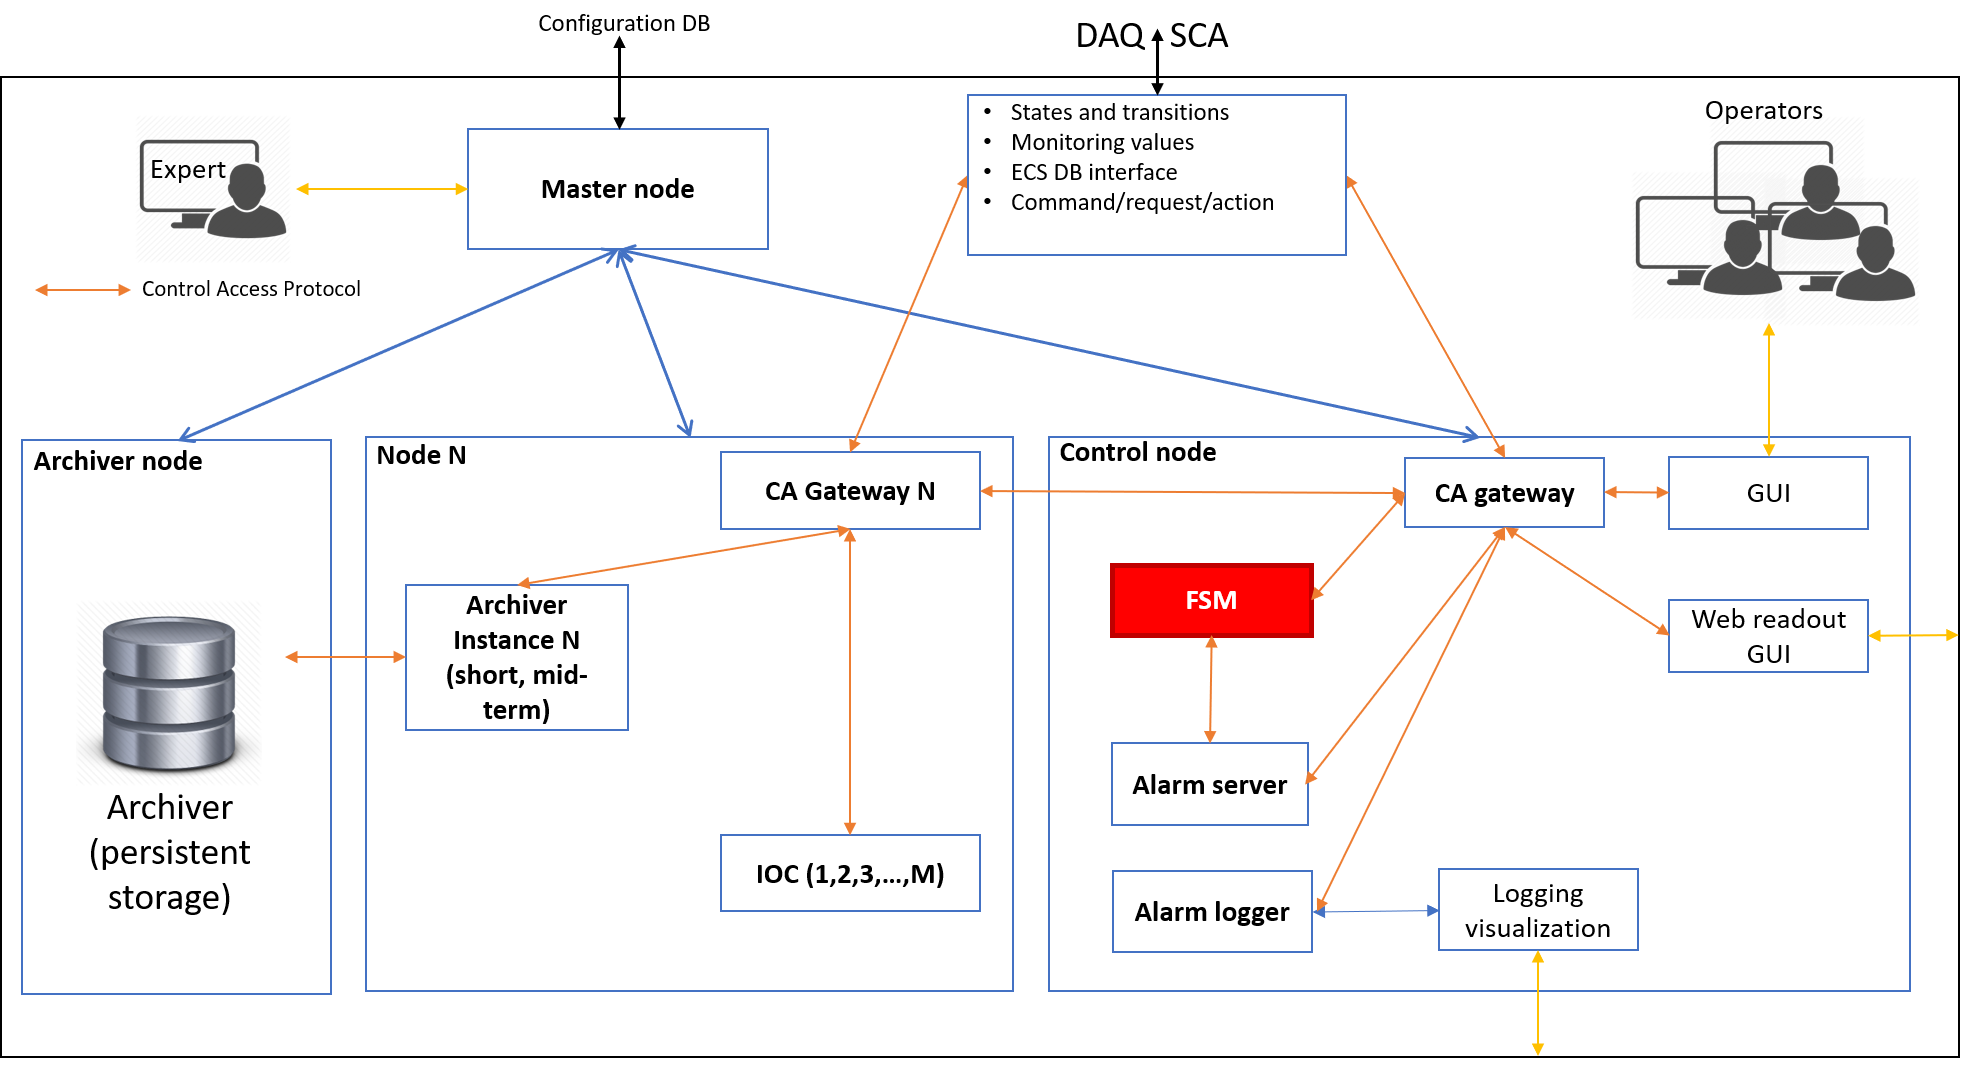
\includegraphics[width=0.85\columnwidth]{Chapter3/Controls/images/DCS.png}
\caption{Proposed \gls{DCS} infrastructure for the \gls{STS}}
\label{fig_arch}
\end{figure}
\newpage





